\chapter{Construction d'une architecture modulaire de cartes auto-organisatrices}


\graphicspath{{03-Algorithme/}}

Le but de cette thèse est de proposer un modèle permettant d'associer des cartes auto-organisatrices dans n'importe quel type d'architecture, comme une sorte de brique de base. En particulier, on cherchera à construire des architectures non-hiéarchiques de cartes, exemple en figure~\ref{fig:archi_non_hierarchique}.
Nous nous placons donc dans le cadre de modules pré-établis, dont les entrées ont été connectées par avance. Les poids de chaque carte seront quant à eux appris, avec comme objectif que les cartes apprennent leurs entrées mais puissent également distinguer un état global de l'architecture.
Pour les entrées, nous nous placons dans un cadre de multi-modalité, détaillé au chapitre suivant. Les différentes cartes prendront des données d'entrées sur différents espaces.

\begin{figure}
\centering
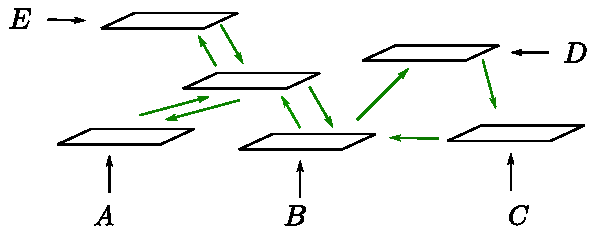
\includegraphics[width=0.6\textwidth]{architecture.pdf}
\caption{Exemple d'architecture modulaire \emph{non-hiérarchique} de cartes de Kohonen. Les entrées sont $A,B,C,D,E$ quelconques. Chaque carte peut ou non prendre une entrée ; les connexions sont réciproques ou non.}
\label{fig:archi_non_hierarchique}
\end{figure}
%\begin{figure}
%\centering
%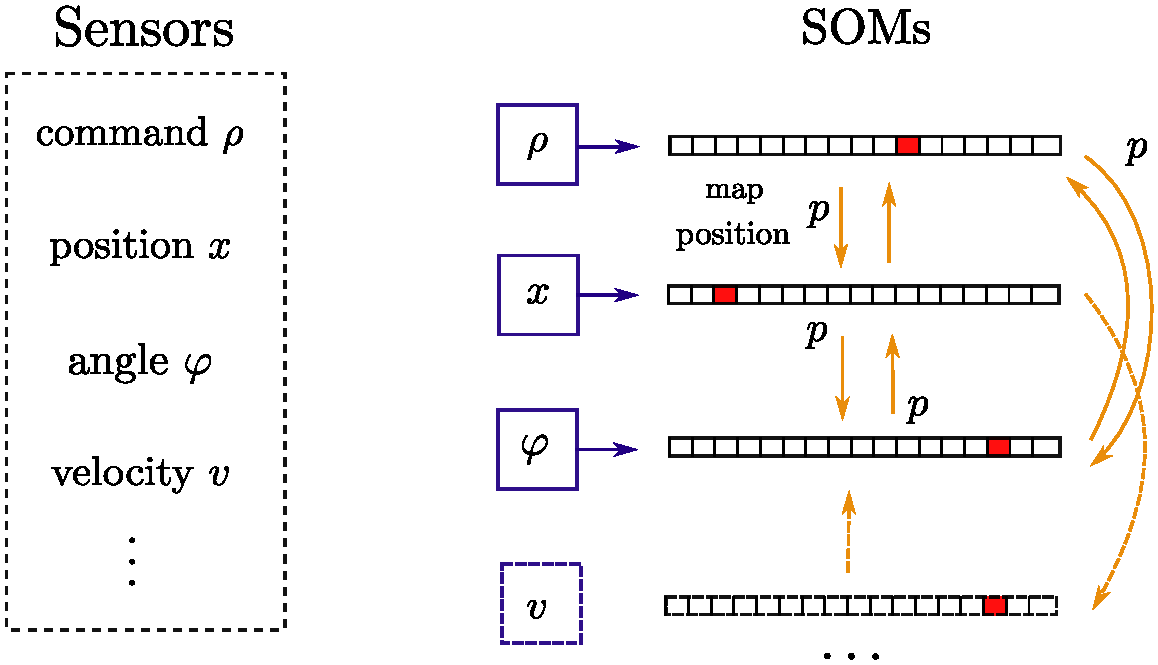
\includegraphics[width=0.6\textwidth]{simplicity.pdf}
%
%\caption{Le but du modèle est de pouvoir assembler des cartes de façon simple, indépendamment du type d'entrée fournie et du nombre de connexions de la carte dans l'architecture. L'ajout de connexions doit aussi pouvoir être réalisé facilement. Cette figure présente un exemple d'architecture de 4 cartes, prenant des entrées différentes et connectées entre elles.}
%\label{fig:simplicity}
%\end{figure}

\section{Description de l'algorithme}

\subsection{Carte de Kohonen classique}

Rappelons les notations concernant une carte de Kohonen standard. Prenons un ensemble de données d'entrées, dans lequel chaque élément est un vecteur d'un espace $D$. On a définit une distance $d$ sur $D$, généralement la distance euclidienne.
La carte de Kohonon construite sur ces entrées est un graphe, généralement une ligne 1D ou une grille 2D de $N$ noeuds. Chaque noeud possède un poids associé $\w_e in D$ ou \emph{prototype}, du même espace que les entrées. et une \emph{position} $i$ dans la carte. Ces positions sont ensuite indexées entre $0$ et $1$ par $p= \frac{i}{N}$ pour l'homogénéité des calculs. 
L'ensemble des poids est noté ${\w_e(p), p \in [0,1]}$. 
L'algorithme se décompose de la façon suivante :

\begin{enumerate}
\item Une entrée $\inpx_t$ est présentée à la carte.
\item L'unité ayant le poids le plus proche de $\inpx_t$ selon la distance $d$ est choisie comme \emph{Best Matching Unit} de la carte. Sa position est notée $\bmu$.
\item Chaque poids $\w_e$ est déplacé vers l'entrées $\inpx$, en fonction de sa distance dans la carte à la best matching unit : 
\begin{equation}
\w_e(p,t+1) = \w_e(p,t) + \alpha h(\bmu,p)(\inpx - \w_e(p,t))
\label{eq:update}
\end{equation}

\end{enumerate}

$h(\bmu,p)$ est la \emph{fonction de voisinage}. Elle est maximale en $p = \bmu$ et décroissante autour de cette position. Dans notre étude, les fonctions de voisinage sont triangulaire, donc maximale en $\bmu$, décroissante sur le rayon de voisinage $h_e$ et nulle après.

Lors de l'étape 2 de l'algorithme, une activité peut être calculée, au lieu d'une distance pour choisir le BMU. Ce dernier est alors choisi comme $\bmu = \argmax_p (a(\inpx,p)$. Nous utiliserons cette solutions dans notre modèle. Les notations au sein d'une carte sont résumées en figure~\ref{fig:one_map_not}.

\begin{figure}
\centering
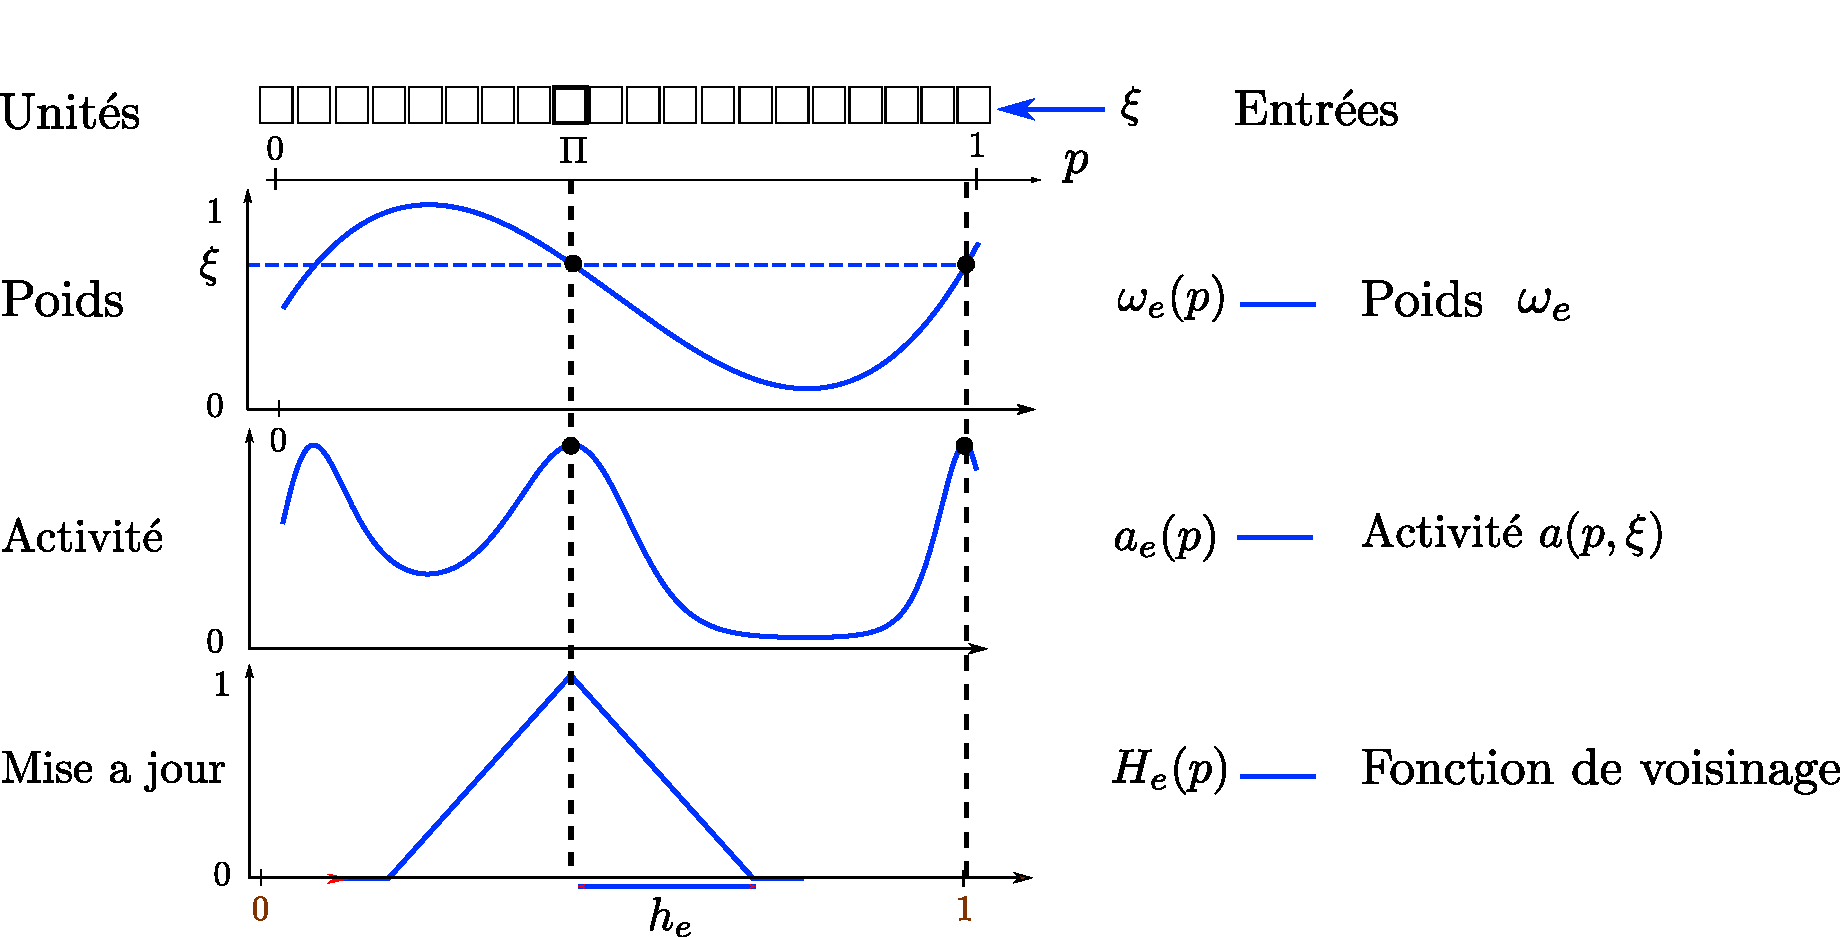
\includegraphics[width=0.6\textwidth]{one_map_one_layer.pdf}
\caption{Notations utilisées dans une carte de Kohonen simple}
\label{fig:one_map_not}
\end{figure}

\subsection{Modèle : CxSOM}

Décrivons maintenant le modèle CxSOM étudié dans cette thèse. Dans ce modèle, l'algorithme original de Kohonen est modifié afin de connecter des cartes entre elles, et d'autoriser des connexions non-hiérarchiques.
Définissons la connexion entre deux cartes. Une carte A est connectée à une carte B lorsque la carte B prend en entrée la position du BMU de la carte A. 
Considérons G, le graphe de connexions des cartes. Ce graphe est \emph{orienté} et les \emph{boucles} sont autorisées. C'est ce qu'on appelera \emph{architecture non-hiérarchique} de cartes, par opposition à des architectures comme HSOM dans laquelle le BMU d'une carte A nourrit une carte B de façon unidirectionnelle. 
Chaque carte aura ainsi plusieurs entrées : une entrée \emph{externes} dans un espace d'entrée, facultative, et $k$ entrées \emph{contextuelles} qui sont les positions des BMU des cartes qui lui sont connectées. Par ailleurs, la recherche du BMU doit être modifiée par rapport à l'originale : les rétroactions entre les cartes sont autorisées, la position du BMU de la carte A va donc influencer la position du BMU de la carte B, lequel modifie à nouveau le BMU de la carte A, etc. 
Notre algorithme présente donc deux modifications principales : 
\begin{itemize}
\item Les cartes possèdent plusieurs entrées, externes et contextuelles. Le calcul de l'activité est donc modifié afin de prendre en compte ces différentes couches d'entrées.
\item La recherche du BMU est modifiée afin de gérer les rétroactions entre cartes.
\end{itemize}

La description du modèle CxSOM est détaillée en figure~\ref{fig:one_map}, dans un cas ou une carte reçoit deux connexions, et l'algorithme explicité en~\ref{algo:cxsom}.

\begin{algorithm}
  \DontPrintSemicolon 
  \SetKwComment{Comment}{}{}
  \caption{Learning iteration with relaxation process}\label{algo:cxsom}
  \KwInput{$\inpx\m{1}, ... , \inpx\m{K} \leftarrow (o^1, \cdots , o^K)\in \mathcal{D}^1 \times \cdot \times \mathcal{D}^K$}
   $t \leftarrow 0$ \;
   $\forall i , \bmu\m{i} \leftarrow \argmax_p a\ext(\inpx\m{i},p)$\;
  \While {$\mathbf{\bmu}(t) \neq \mathbf{ \bmu}(t-1)$}{
  \ForAll{Map $i$}{
  $\inpc\m{i}_1,...\inpc\m{i}_k \leftarrow$ BMUs from connected maps \;
  Computation of $a_g^i$ (equation~\ref{activity}) \;
  $p\star\m{i} \leftarrow \argmax_p a_g^i(p)$ \;
  $\bmu\m{i} \leftarrow \bmu\m{i} + min(\Delta, \lvert p\star\m{i} - \bmu\m{i} \rvert) \times \sign(p\star\m{i} - \bmu\m{i})$ \;
  }
  $t \leftarrow t+1$ \;
  }
  $\forall i, \w\ext\m{i}(p) \leftarrow \w\ext\m{i}(p) + H\ext(\bmu\m{i}, p)(\w\ext\m{i}(p) - \inpx\m{i})$\;
  $\forall i, \forall k, \w_{ck}\m{i}(p) \leftarrow \w_{ck}\m{i}(p) + H\cont(\bmu\m{i},p)(\w_{ck}\m{i}(p) - \inpc\m{i})$
\end{algorithm}
 
\subsubsection{Gestion des entrées externes et contextuelles}

A un pas d'apprentissage $t$, une carte $M$ reçoit en entrée une entrée \emph{externe} notée $\inpx_t$ et $K$ entrées \emph{contextuelles} notées $\inpc_{0t},\cdots,\inpc_{Kt}$, qui sont les BMU $\bmu$ des cartes qui lui sont connectées. La carte possède donc $k+1$ couches de poids. $\w_e$ correspond à l'entrée externe et $\w_{c0}, \cdots, \w_{cK}$ aux entrées contextuelles. On calcule une activité séparément sur chaque couche de poids selon la formule suivante : 
\begin{equation}
\label{eq:activite}
a(p,x) = \exp(\frac{(\w(p)-x)^2}{2\sigma^2} \; x = \inpx_t\; \text{ou}\; \inpc_{kt}, \; \w = \w_e \;\text{ou}\; \w_{ck}
\end{equation}
Les activités contextuelles sont moyennées en une activité $a_c(p,\mathbf{\inpc}_t)$, avec $\mathbf{\inpc_t} = (\inpc_{0t}, \cdots, \inpc{Kt})$. 
Les activités externes et contextuelles sont enfin fusionnées en une activité globale:
\begin{equation}
\label{eq:global_act}
a_g(p,\inpx_t,\mathbf{\inpc_t}) = \sqrt{a_e(p,\inpx_t)(\beta a_e(p,\inpx_t) + (1-\beta) a_c(p, \mathbf{\inpc_t})}
\end{equation}

Cette activation globale est utilisée pour déterminer le BMU de la carte. 

\subsubsection{Gestion des rétroactions dans l'architecture}

Contrairement à une carte simple, on ne peut pas calculer tous les BMUs de l'architecture en prenant l'argmax de $a_g$ dans chaque carte. A cause des influences mutuelles entre cartes, calculer le BMU d'une des cartes modifie les entrées des autres cartes de l'architecture, et donc leur BMU. Cette recherche est donc réalisée par un processus dynamique que l'on appelera \emph{relaxation}, menant à un consensus entre cartes : on cherche le point, s'il existe, où chaque BMU maximise l'activité globale de chaque carte.

Le processus de relaxation est donc une boucle imbriquée dans un pas d'apprentissage de l'architecture, indexée par $\tau$. Notons $\bmu\m[i]$ la position du BMU de la carte $i$, et $\mathbf{\bmu} = (\bmu\m[0], \cdots , \bmu\m[n])$, avec $n$ le nombre de cartes de l'architecture.
Au début d'un pas d'apprentissage, chaque carte est nourrie avec une entrée externe $\inpx^i_t$, et les activités externes $a_e^i(\inpx^i_t,p)$ de chaque carte peuvent être calculées.
La recherche du BMU suit donc le processus de relaxation suivant : 
\begin{enumerate}
\item Dans chaque carte $i$, la position $\bmu^i$ est initialisée à $\argmax_p(a_e^i(\inpx^i_t,p)$. Les entrées contextuelles sont alors initialisées en prenant le BMU correspondant aux connexions de l'architecture.
\item Tant que toutes les positions $\bmu^i$ ne sont pas stables, 
	\begin{enumerate}
	\item Dans chaque carte $i$, calculer les activités contextuelles et globales, définissant ainsi $p^{\star i} = \argmax_p(a_g(p,\mathbf{\inpc^i},\inpx^i)$
	\item Déplacer $\bmu^i$ vers $p^{\star i}$ : $\bmu^i \leftarrow \bmu^i \pm \Delta$ si $\lvert \bmu^i - p^{\star i} \rvert \geq \Delta$, $\bmu^i \leftarrow p^{\star i}$ sinon
	\end{enumerate}
	
\item Le BMU de chaque carte est pris comme la valeur finale stable de ce processus dynamique. Cette valeur est utilisée pour les mise a jour des poids.
\end{enumerate}

Il peut arriver que les positions se stabilisent sur un cycle limite. Dans ce cas, on arrêtera la relaxation arbitrairement; ce phénomène étant ponctuel, il n'influencera pas l'apprentissage. Les paramètres des cartes de l'architecture sont choisis pour éviter de telles situations.

\begin{figure}
\centering
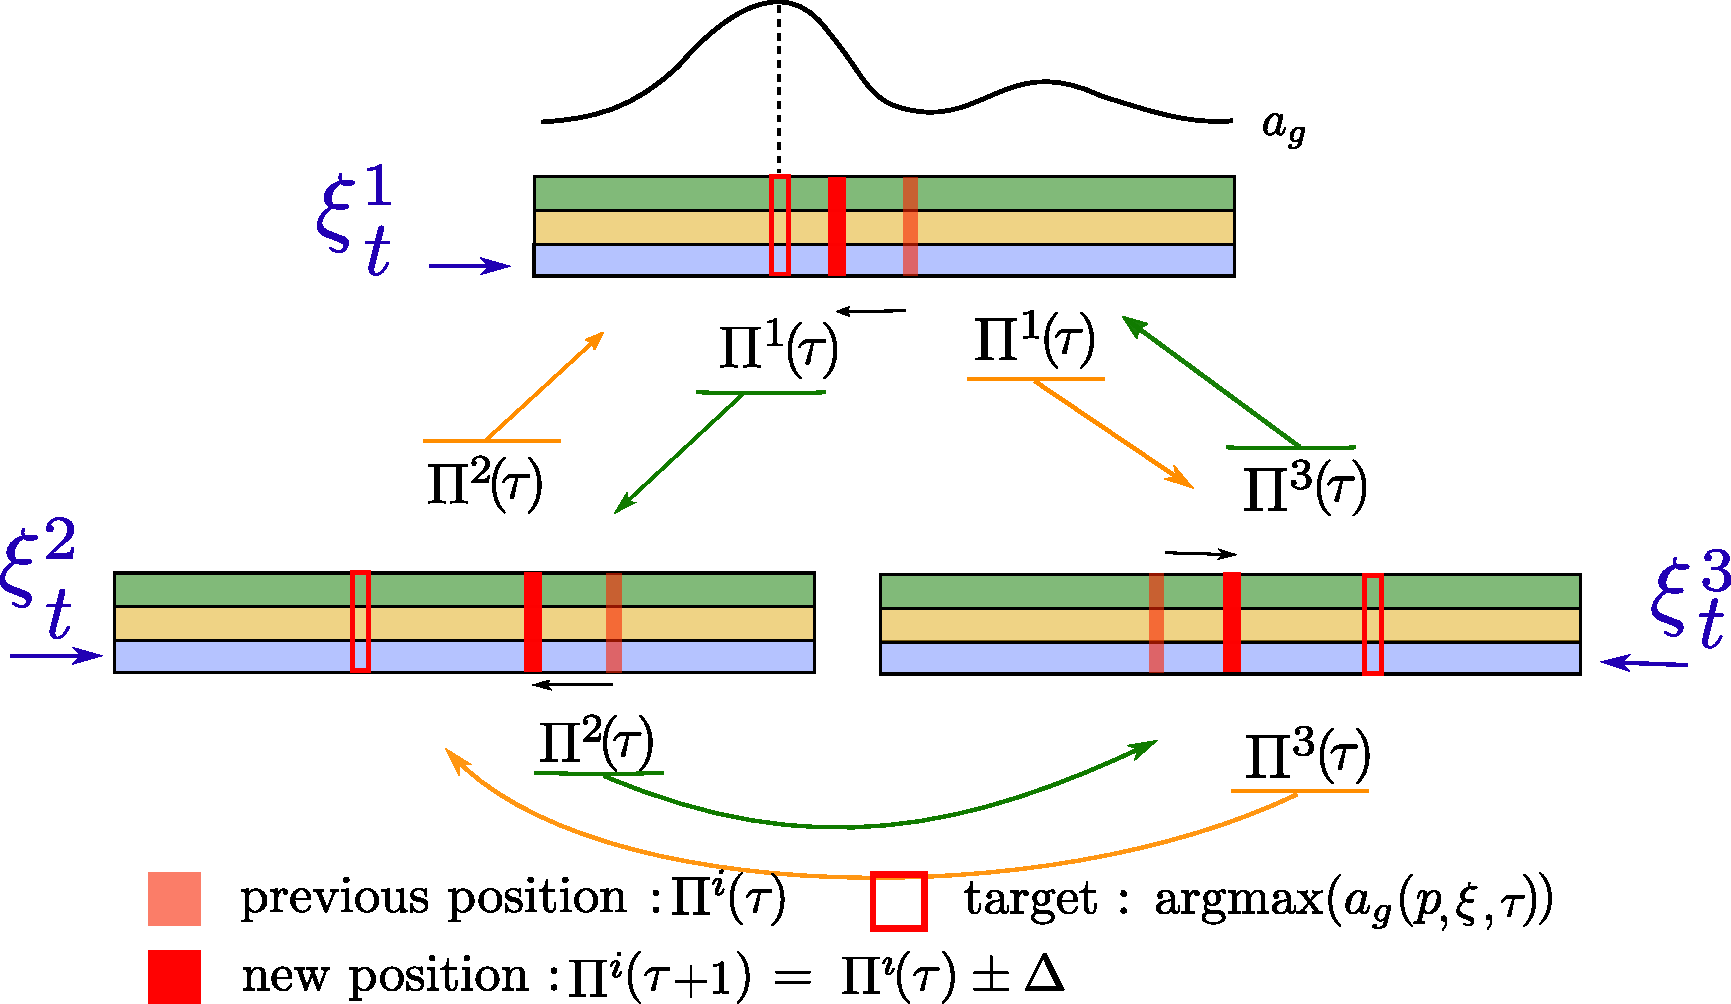
\includegraphics[width=0.6\textwidth]{relaxation.pdf}
\label{fig:relax}
\caption{description d'une étape de la relaxation dans l'architecture, aboutissant à un consensus entre cartes. Au sein d'une même itération $t$, les position des BMU $\bmu$ sont légèrement déplacées jusqu'à ce que toutes les positions $\bmu$ des cartes de l'architecture soient stable. Ces positions maximisent collectivement les activités globales de chaque carte. }
\end{figure}

\begin{figure}
\centering
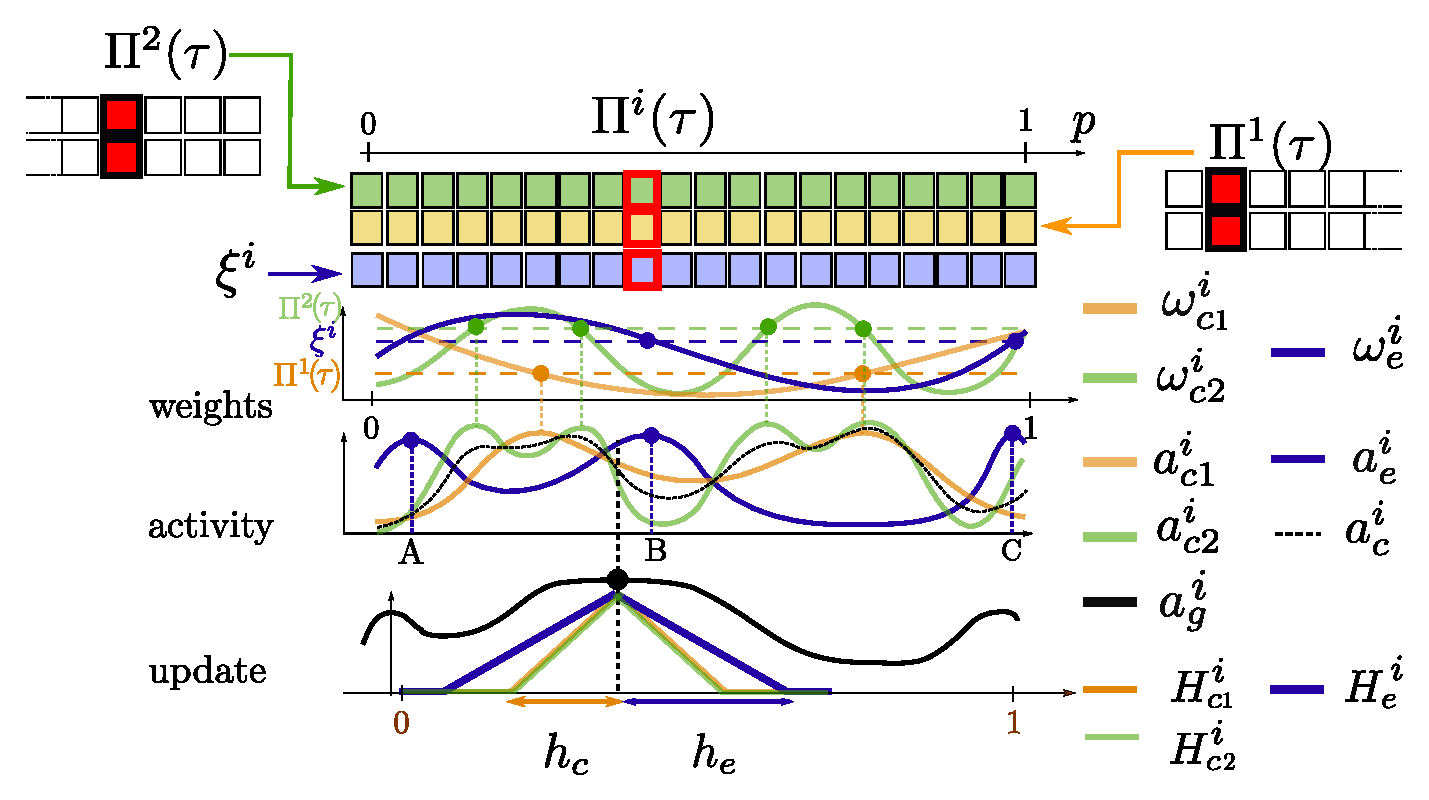
\includegraphics[width=0.8\textwidth]{one_map.pdf}
\caption{Description d'une carte au sein d'une architecture CxSOM. La carte recoit deux connexions de cartes voisines, et possède donc deux couches contextuelles}
\label{fig:one_map}
\end{figure}

\subsubsection{Mise à jour des poids}

Les poids sont mis à jour par rapport à leurs entrées respectives suivant l'équation \ref{eq:update}. Le BMU d'une carte est ainsi commun à toutes les couches. Les rayons de voisinage $h_e$ et $h_c$ ont des valeurs différentes ; celles-ci seront détaillée en partie suivante. 

\subsubsection{Tests}

Les expériences faites sur l'architecture se décomposent en une phases d'apprentissage et phases de test. Pendant les tests, la mise à jour des poids des cartes est gelée et seuls le calcul des activités et le processus dynamique de sélection du BMU sont effectués.

\section{Choix des paramètres}

\subsection{Influence des rayons de voisinage}

\subsection{Influence des autres paramètres}

\subsection{Compatibilité en 2D}

\section{Analyse de la relaxation}

L'apprentissage conjoint des cartes repose sur la relaxation au sein d'une itération. On cherche donc à vérifier si la relaxation converge vers une valeur quelle que soit l'entrée, et si elle est pertinente en large dimension avec de nombreuses cartes.

\subsection{Analyse expérimentale}

\subsection{Champs de BMU}

\subsection{Limitations et possibilités en grande dimension}

\section{Implémentation}
L'histoire de la recherche de consensus dans le graphe de cartes, permet que ce soit vraiment décentralisé

\section{Perspectives d'évolutions}